\chapter{Materiais e Métodos}
\label{cap:03}
Para a aquisição de dados foram utilizados diversos conceitos e ferramentas eletrônicas de diversas esferas específicas, garantindo uma melhor adaptação para o objetivo específico de traçador IxV.%ADICIONAR REFERÊNCIAS SOBRE O PROTÓTIPO

\section{Arduino}
Arduino, plataforma \textit{open-source}, baseada em fácil prototipagem eletrônica e de programação, permite o fácil e rápido desenvolvimento de protótipos. Devido a fácil disponibilidade no mercado e alto custo x benefício, fez-se o uso do Arduino Uno como componente principal para o controle e aquisição de dados para a curva IxV.

\FloatBarrier
\begin{figure}[!htbp]
	\centering
	%scale redimensiona a figura.
	%1.5 = 150% do tamanho original
	%1 = 100% do tamanho original
	%0.20 = 20% do tamanho original
	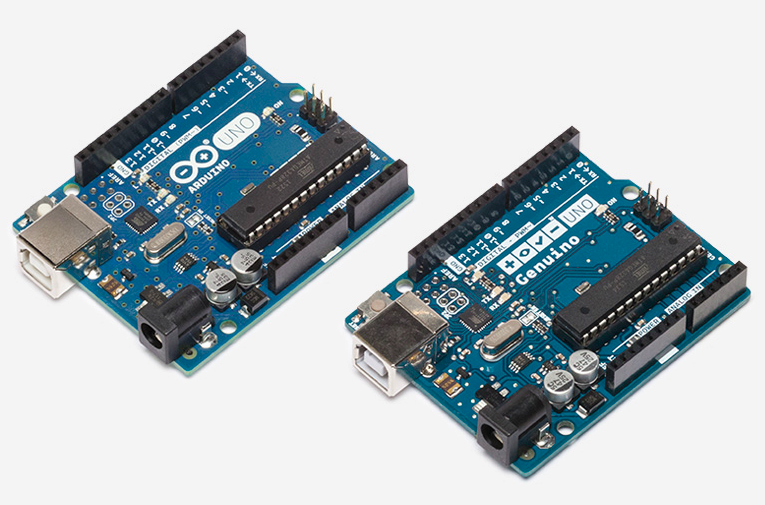
\includegraphics[scale=0.7]{imagens/Uno}
	\caption{Exemplos de Arduinos Uno. Fonte:  \url{https://www.arduino.cc/en/Guide/ArduinoUno}. }
	
	\label{fig:ArduinoUno}
\end{figure}
\FloatBarrier

Na Tabela 2 São Listadas as principais características encontradas no hardware do Arduino Uno.

\FloatBarrier
\begin{table}[!htbp]
	\centering
	\caption{Tabela do hardware do Arduino Uno}
	\begin{tabular}{ c | c }
		\hline
		Microcontrolador                & ATmega328P                                            \\ \hline
		Tensão operacional              & 5V                                                    \\ \hline
		Tensão de entrada (recomendado) & 7-12V                                                 \\ \hline
		Pinos Digital I / O             & 6-20V                                                 \\ \hline
		PWM Digital I / O Pins          & 6                                                     \\ \hline
		Pinos de entrada analógica      & 6                                                     \\ \hline
		Corrente DC por pino de E / S   & 20 mA                                                 \\ \hline
		Corrente DC para Pin 3.3V       & 50 mA                                                 \\ \hline
		Memória flash                   & 32 KB (ATmega328P) \\ \hline
		SRAM                            & 2 KB (ATmega328P)                                     \\ \hline
		EEPROM                          & 1 KB (ATmega328P)                                     \\ \hline
		Velocidade do relógio           & 16 MHz                                                \\ \hline
		LED BUILTIN                     & 13                                                    \\ \hline
		comprimento                     & 68.6 mm                                               \\ \hline
		Largura                         & 53.4 mm                                               \\ \hline
		Peso                            & 25 g                                                  \\ \hline
	\end{tabular}
	\\ \vspace{0.2cm}
	\textbf{Fonte:} Adaptado de \url{https://store.arduino.cc/usa/arduino-uno-rev3} .
	\label{tab:ArduinoUno}
\end{table}
\FloatBarrier

Conforma mostrado na tabela~\ref{tab:ArduinoUno}, o Arduino Uno possui 6 entradas analógicas, entretanto há grande imprecisão nestas entradas. De forma a garantir maior precisão nas coletas de dados, foi utilizado um modulo conversor analógico.

\section{ADS1115}
O módulo ADS1115 da Adafruit é um módulo ADC com resolução de 16-Bits e utiliza a comunicação I2C, o uso deste módulo foi vital para a aquisição de dados.

Diferentemente dos conversores Analógico Digital integrados na placa Arduino, o módulo ADS1115 possui ótima repetibilidade e grande precisão durante a a aquisição dos valores.

Há ainda a possibilidade do uso de amplificadores internos através de FPGA de forma a aumentar ainda mais a precisão das medidas.

Ao se utilizar sua resolução de 16-Bits, e ganho unitário é possível obter-se uma precisão de 0,125 $mV$, o qual ultrapassa grandemente o fundo de escala de 4,9 $mV$ do ADC proveniente do Arduino.%ADICIONAR REFERÊNCIA DE ONDE TIROU OS DADOS
\FloatBarrier
\begin{figure}[!htbp]
	\centering
	%scale redimensiona a figura.
	%1.5 = 150% do tamanho original
	%1 = 100% do tamanho original
	%0.20 = 20% do tamanho original
	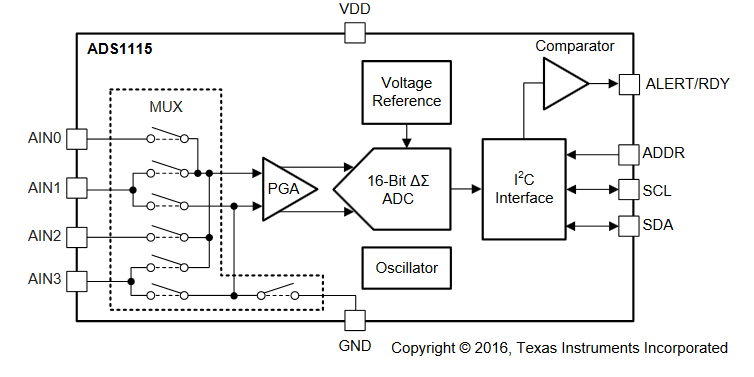
\includegraphics[scale=0.7]{imagens/ADS}
	\caption{Diagrama de blocos. Fonte: Datasheet do fabricante. }%ADICIONAR DATASHEET COM OS DADOS DO ARDUINO.
	
	\label{fig:Ads}
\end{figure}
\FloatBarrier
